% ============================================================
%  Real-Time EV CAN Bus Simulation — Major Project Report
%  Author  : Mohammed Rayan
%  Org     : Ary's Garage — Electronics / EEE 2026
%  Engine  : pdfLaTeX (compile twice for ToC + cross-refs)
%  Upload  : Overleaf — no external image files required
% ============================================================

\documentclass[12pt, a4paper, openany]{report}

% ── Encoding & Base Font ─────────────────────────────────────
\usepackage[T1]{fontenc}
\usepackage[utf8]{inputenc}
\usepackage{lmodern}
\usepackage{microtype}

% ── Page Layout ─────────────────────────────────────────────
\usepackage[
  top    = 2.5cm,  bottom = 2.5cm,
  left   = 3.0cm,  right  = 2.5cm,
  headheight = 15pt
]{geometry}

% ── Colour Palette ──────────────────────────────────────────
\usepackage[dvipsnames, table, x11names]{xcolor}
\definecolor{Navy}      {RGB}{12,  28,  70}
\definecolor{Royal}     {RGB}{0,   90, 200}
\definecolor{LightBlue} {RGB}{220, 235, 255}
\definecolor{CodeBg}    {RGB}{247, 249, 252}
\definecolor{DkGray}    {RGB}{55,  55,  65}
\definecolor{MidGray}   {RGB}{135, 135, 145}
\definecolor{GreenOK}   {RGB}{0,  155,  70}
\definecolor{Amber}     {RGB}{215, 120,   0}
\definecolor{TblHead}   {RGB}{12,  28,  70}
\definecolor{TblAlt}    {RGB}{233, 241, 255}

% ── Hyperlinks ───────────────────────────────────────────────
\usepackage[
  colorlinks = true,
  linkcolor  = Royal,
  citecolor  = Royal,
  urlcolor   = Royal,
  pdftitle   = {Real-Time EV CAN Bus Simulation with Live Dashboard},
  pdfauthor  = {Mohammed Rayan},
  bookmarks  = true,
  bookmarksopen = true
]{hyperref}

% ── Header / Footer ──────────────────────────────────────────
\usepackage{fancyhdr}
\pagestyle{fancy}
\fancyhf{}
\fancyhead[L]{\small\color{DkGray}\itshape EV CAN Bus Simulation}
\fancyhead[R]{\small\color{DkGray}\itshape Mohammed Rayan \ $|$ \ Ary's Garage}
\fancyfoot[C]{\small\color{MidGray}\thepage}
\renewcommand{\headrulewidth}{0.5pt}
\renewcommand{\headrule}{%
  {\color{Royal}\hrule width\headwidth height 0.5pt}}
\renewcommand{\footrulewidth}{0pt}

% ── Chapter / Section Styling ────────────────────────────────
\usepackage{titlesec}
\usepackage{needspace}

% Make chapters flow inline (no forced page break) — eliminates white gaps
\titleclass{\chapter}{straight}

% Chapter: large coloured title with a 2 pt rule beneath
\titleformat{\chapter}[block]
  {\normalfont\huge\bfseries\color{Navy}}
  {\color{Royal}\thechapter.}{0.6em}{}
  [{\color{Royal}\titlerule[2pt]}]
\titlespacing*{\chapter}{0pt}{28pt}{18pt}

% Section
\titleformat{\section}
  {\normalfont\Large\bfseries\color{Navy}}
  {\thesection}{1em}{}
  [{\color{Royal!55}\titlerule[0.7pt]}]
\titlespacing*{\section}{0pt}{16pt}{6pt}

% Subsection
\titleformat{\subsection}
  {\normalfont\large\bfseries\color{DkGray}}
  {\thesubsection}{1em}{}
\titlespacing*{\subsection}{0pt}{10pt}{4pt}

% Subsubsection
\titleformat{\subsubsection}
  {\normalfont\normalsize\bfseries\color{DkGray}}
  {\thesubsubsection}{1em}{}
\titlespacing*{\subsubsection}{0pt}{8pt}{2pt}

% ── Math ─────────────────────────────────────────────────────
\usepackage{amsmath}
\usepackage{amssymb}

% ── Tables ───────────────────────────────────────────────────
\usepackage{booktabs}
\usepackage{tabularx}
\usepackage{array}
\usepackage{multirow}
\usepackage{makecell}
\renewcommand{\arraystretch}{1.18}
\setlength{\tabcolsep}{6pt}
% Tighter float placement — less blank space around floated tables
\setlength{\textfloatsep}{8pt plus 2pt minus 4pt}
\setlength{\floatsep}{6pt plus 2pt minus 2pt}
\setlength{\intextsep}{6pt plus 2pt minus 2pt}

% ── Code Listings ────────────────────────────────────────────
\usepackage{listings}

\lstdefinestyle{python}{
  language         = Python,
  backgroundcolor  = \color{CodeBg},
  basicstyle       = \footnotesize\ttfamily\color{Navy},
  keywordstyle     = \bfseries\color{Royal},
  commentstyle     = \itshape\color{MidGray},
  stringstyle      = \color{GreenOK},
  numberstyle      = \tiny\color{MidGray},
  numbers          = left,
  numbersep        = 9pt,
  breaklines       = true,
  frame            = single,
  framesep         = 5pt,
  rulecolor        = \color{Royal!35},
  xleftmargin      = 18pt,
  xrightmargin     = 5pt,
  tabsize          = 2,
  showstringspaces = false,
  captionpos       = b,
}
\lstdefinestyle{shell}{
  backgroundcolor  = \color{Navy!7},
  basicstyle       = \scriptsize\ttfamily\color{Navy},
  breaklines       = true,
  frame            = single,
  framesep         = 5pt,
  rulecolor        = \color{Royal!35},
  numbers          = none,
  xleftmargin      = 10pt,
  xrightmargin     = 5pt,
  showstringspaces = false,
}
\lstset{style=shell}

% ── TikZ ─────────────────────────────────────────────────────
\usepackage{tikz}
\usetikzlibrary{shapes.geometric, arrows.meta, positioning,
                fit, backgrounds, calc, shadows.blur, decorations.pathreplacing}

% ── Misc Packages ────────────────────────────────────────────
\usepackage{graphicx}
\usepackage{float}
\usepackage[section]{placeins}
\usepackage{setspace}
\usepackage{parskip}
\usepackage{enumitem}
\usepackage{caption}
\usepackage{tcolorbox}
\tcbuselibrary{skins, breakable}

\captionsetup{
  labelfont = {bf, color=Navy},
  textfont  = {small, color=DkGray},
  labelsep  = period,
}

% ── Custom Environments ──────────────────────────────────────
\newtcolorbox{infobox}[1][]{
  enhanced, breakable,
  colback  = LightBlue,
  colframe = Royal,
  coltitle = white,
  fonttitle= \bfseries\small,
  title    = #1,
  left = 7pt, right = 7pt, top = 5pt, bottom = 5pt,
}
\newtcolorbox{resultbox}{
  enhanced,
  colback  = GreenOK!9,
  colframe = GreenOK,
  left = 7pt, right = 7pt, top = 5pt, bottom = 5pt,
}

% ── Global Spacing ───────────────────────────────────────────
\setlength{\parindent}{0pt}
\setlength{\parskip}{6pt}
\onehalfspacing
\raggedbottom

% ── Convenience ──────────────────────────────────────────────
\newcommand{\code}[1]{\texttt{#1}}
\newcommand{\degree}{$^\circ$}
\newcommand{\ohm}{$\Omega$}

% =============================================================
%  DOCUMENT BEGIN
% =============================================================
\begin{document}

% ─────────────────────────────────────────────────────────────
%  TITLE PAGE
% ─────────────────────────────────────────────────────────────
\begin{titlepage}
\pagecolor{Navy}
\color{white}


\begin{tikzpicture}[remember picture, overlay]
  %% Top accent bar
  \fill[Royal] (current page.north west)
    rectangle ([yshift=-3.2cm] current page.north east);
  %% Bottom accent bar
  \fill[Royal!60!Navy] (current page.south west)
    rectangle ([yshift=2.2cm] current page.south east);
  %% Subtle diagonal watermark stripe
  \fill[white, opacity=0.025]
    ([xshift=12cm] current page.south west) --
    ([xshift=18cm] current page.south west) --
    ([xshift=18cm, yshift=29.7cm] current page.south west) --
    ([xshift=12cm, yshift=29.7cm] current page.south west) -- cycle;
  %% Right-edge thin stripe
  \fill[Royal!40, opacity=0.5]
    ([xshift=-0.8cm] current page.north east) rectangle
    (current page.south east);
\end{tikzpicture}

\vspace*{3.0cm}

\begin{center}

  {\large\bfseries\color{white!70}\MakeUppercase{%
    Ary's Garage \enspace---\enspace Electronics / EEE Assignment 2026}}

  \vspace{0.5cm}
  {\color{Royal!70}\rule{13cm}{0.6pt}}
  \vspace{0.7cm}

  {\fontsize{30}{38}\selectfont\bfseries
    Real-Time Electric Vehicle\\[0.35cm]
    CAN Bus Simulation\\[0.35cm]
    with Live Dashboard}

  \vspace{0.7cm}
  {\color{Royal!70}\rule{13cm}{0.6pt}}
  \vspace{1.4cm}

  \begin{tabular}{r@{\quad}l}
    \color{white!55}\textbf{Candidate}    & \textbf{Mohammed Rayan} \\[5pt]
    \color{white!55}\textbf{Email}        & mohammedrah1289@gmail.com \\[5pt]
    \color{white!55}\textbf{Repository}   & arys-eee-can-sim \\[5pt]
    \color{white!55}\textbf{Category}     & Electronics / EEE \\[5pt]
    \color{white!55}\textbf{Language}     & Python 3.11 \\[5pt]
    \color{white!55}\textbf{Deadline}     & 5 June 2026, 10:00\,AM IST \\[5pt]
    \color{white!55}\textbf{Submit to}    & future@arysgarage.com \\
  \end{tabular}

\end{center}

\vfill

\begin{center}
  \color{white!40}{\small
    Subject: Assignment Submission --- Mohammed Rayan ---
    Real-Time EV CAN Bus Simulation}
\end{center}

\vspace*{0.6cm}
\end{titlepage}

\pagecolor{white}
\color{black}
\setcounter{page}{1}

% ─────────────────────────────────────────────────────────────
%  ABSTRACT PAGE (standalone, unnumbered)
% ─────────────────────────────────────────────────────────────
\chapter*{Abstract}
\addcontentsline{toc}{chapter}{Abstract}
\thispagestyle{fancy}

This project implements a fully functional, real-time simulation of the CAN
(Controller Area Network) communication architecture used in modern Battery
Electric Vehicles (BEVs). Three software-defined Electronic Control Units
(ECUs)~--- a Battery Management System (BMS), a Vehicle Control Unit (VCU),
and a Motor Control Unit (MCU)~--- communicate over a virtual CAN~2.0A bus
using a real DBC file parsed by the \code{cantools} library.

The battery is modelled as a first-order Thevenin Equivalent Circuit Model
(1RC ECM) with an OCV--SOC lookup table, RC branch dynamics solved via exact
exponential integration, and a coupled thermal model. Vehicle longitudinal
dynamics follow Newton's second law with aerodynamic drag, rolling
resistance, and braking. Each ECU runs as an independent asyncio coroutine
with its own inbox queue (actor model), finite state machine (FSM), watchdog
timer, and ISO~14229 UDS handler.

Advanced features include a pre-charge FSM with RC capacitor physics
modelling the DC link voltage ramp before main contactor closure; four fault
injection modes (CAN wire cut, CRC corruption, thermal runaway, overspeed);
an ISO~26262 ASIL-B plausibility check cutting torque on simultaneous
throttle-and-brake; discharge current clamping at both the MCU and physics
layers; and a real-time WebSocket dashboard with Chart.js telemetry. All
simulated CAN traffic can be exported as a CANalyzer-compatible \code{.asc}
file readable in Vector~CANalyzer, PEAK~PCAN-Explorer, and the \code{cantools}
CLI.

\smallskip

\begin{resultbox}
\textbf{Summary of outcomes:} All 8 end-to-end runbook scenarios pass.
All 6 automated \code{pytest} tests pass (0.73\,s total). Three layers of
safety protection prevent runaway states in any operating condition.
Two features beyond the base specification --- a pre-charge FSM and
CANalyzer \code{.asc} export --- demonstrate real EV hardware awareness.
\end{resultbox}

\smallskip

\begin{center}
\begin{tabular}{llp{5.5cm}}
  \toprule
  \rowcolor{TblHead}
  \color{white}\textbf{Metric} &
  \color{white}\textbf{Value} &
  \color{white}\textbf{Notes} \\
  \midrule
  Runbook scenarios         & 8 / 8 passed   & End-to-end live dashboard \\
  \rowcolor{TblAlt}
  Automated tests           & 6 / 6 passed   & pytest-asyncio, 0.73\,s \\
  ECUs simulated            & 3              & BMS, VCU, MCU \\
  \rowcolor{TblAlt}
  CAN messages              & 4              & 14 signals, real DBC file \\
  Physics time step         & 10\,ms         & Drift-free scheduler \\
  \rowcolor{TblAlt}
  Pre-charge time ($\tau$)  & 0.5\,s         & 90\% threshold at $\approx$1.15\,s \\
  .asc export log           & 50\,000 frames & $\approx$10\,min at full rate \\
  \bottomrule
\end{tabular}
\end{center}

\clearpage

% ─────────────────────────────────────────────────────────────
%  TABLE OF CONTENTS
% ─────────────────────────────────────────────────────────────
\tableofcontents
\clearpage

% =============================================================
%  CHAPTER 1 — TITLE & CANDIDATE DETAILS
% =============================================================
\chapter{Title \& Candidate Details}

\begin{center}
\begin{tabularx}{0.88\textwidth}{lX}
  \toprule
  \rowcolor{TblHead}
  \color{white}\textbf{Field} &
  \color{white}\textbf{Detail} \\
  \midrule
  Project Title       & Real-Time Electric Vehicle CAN Bus Simulation with Live Dashboard \\
  \rowcolor{TblAlt}
  Assignment Category & Electronics / EEE \\
  Candidate Name      & Mohammed Rayan \\
  \rowcolor{TblAlt}
  Email               & mohammedrah1289@gmail.com \\
  GitHub Repository   & arys-eee-can-sim \\
  \rowcolor{TblAlt}
  Primary Language    & Python 3.11 \\
  Submission Deadline & 5 June 2026, 10:00 AM IST \\
  \rowcolor{TblAlt}
  Organisation        & Ary's Garage \\
  Submission Address  & future@arysgarage.com \\
  \bottomrule
\end{tabularx}
\end{center}

% =============================================================
%  CHAPTER 2 — ABSTRACT (numbered)
% =============================================================
\chapter{Abstract}

See the unnumbered Abstract page preceding the Table of Contents for the
full abstract. In summary:

\begin{itemize}[leftmargin=1.5em]
  \item Three asyncio-based ECUs (BMS, VCU, MCU) communicate over a virtual
        CAN~2.0A bus using a real DBC file.
  \item The battery is a 1RC Thevenin ECM with exact exponential RC
        integration, OCV--SOC interpolation, and a coupled thermal model.
  \item The BMS implements a pre-charge FSM (INIT $\to$ PRECHARGE $\to$
        ACTIVE) with RC capacitor physics ($\tau = 0.5$\,s).
  \item ISO~14229 UDS services 0x22, 0x19, and 0x14 are implemented on all
        three ECUs.
  \item ISO~26262 ASIL-B plausibility check, watchdog timers, and dynamic
        current derating protect against unsafe states.
  \item All simulated traffic exports to CANalyzer \code{.asc} format.
  \item \textbf{Result:} 8/8 runbook scenarios passed, 6/6 automated tests
        passed.
\end{itemize}

% =============================================================
%  CHAPTER 3 — TOOLS & AI USAGE
% =============================================================
\chapter{Tools \& AI Usage}

\section{Software Tools}

\begin{center}
\begin{tabularx}{\textwidth}{llX}
  \toprule
  \rowcolor{TblHead}
  \color{white}\textbf{Tool} &
  \color{white}\textbf{Version} &
  \color{white}\textbf{Purpose} \\
  \midrule
  Python          & 3.11   & Primary simulation language \\
  \rowcolor{TblAlt}
  FastAPI         & 0.111  & REST API and WebSocket server \\
  uvicorn         & 0.29   & ASGI server (Thread~2) \\
  \rowcolor{TblAlt}
  cantools        & 39.x   & DBC file parsing, CAN frame encode/decode \\
  NumPy           & 1.26   & OCV--SOC interpolation (\code{np.interp}) \\
  \rowcolor{TblAlt}
  Pydantic v2     & 2.x    & YAML configuration validation at startup \\
  PyYAML          & 6.x    & YAML configuration loading \\
  \rowcolor{TblAlt}
  pytest          & 8.x    & Automated test suite (6 tests) \\
  pytest-asyncio  & 0.23   & Async test support \\
  \rowcolor{TblAlt}
  Chart.js        & 4.4    & Real-time telemetry chart in dashboard \\
  WebSocket API   & ---    & Live bidirectional dashboard communication \\
  \bottomrule
\end{tabularx}
\end{center}

\section{AI Tools Used}

\textbf{Tool:} Claude (Anthropic), accessed via Claude Code CLI.

\subsection{Scope of AI Assistance}

AI assistance was used selectively across four areas of the project.
In each case the AI served as a reference and sounding board rather than
a primary author; all design decisions, implementation choices, and
verification were carried out by the candidate.

\begin{center}
\begin{tabularx}{\textwidth}{lXl}
  \toprule
  \rowcolor{TblHead}
  \color{white}\textbf{Area} &
  \color{white}\textbf{Nature of Assistance} &
  \color{white}\textbf{Extent} \\
  \midrule
  System architecture
    & Discussed the two-thread separation (asyncio vs.\ uvicorn) and
      cross-thread data-passing constraints; final structure designed
      and implemented by candidate.
    & Partial \\
  \rowcolor{TblAlt}
  Physics \& dynamics
    & Consulted on the 1RC Thevenin ECM formulation and exponential RC
      integration stability; vehicle dynamics equations verified against
      standard references with AI as a secondary check.
    & Partial \\
  Debugging
    & Used to help trace two runtime issues (bus-reference scope,
      current clamping direction); root-cause analysis and fix
      authored by candidate.
    & Partial \\
  \rowcolor{TblAlt}
  Report preparation
    & Used for structural suggestions and language review of the written
      sections; all technical content, data, and conclusions written
      by candidate.
    & Partial \\
  \bottomrule
\end{tabularx}
\end{center}

All code was written, tested, and validated independently by the candidate.
AI suggestions were reviewed critically and were not applied verbatim;
where an AI suggestion conflicted with project requirements or test results,
the candidate's judgement took precedence.

% =============================================================
%  CHAPTER 4 — DESIGN & METHODOLOGY
% =============================================================
\chapter{Design \& Methodology}

\section{System Architecture}

The simulation is split across two OS threads that share data only through
\code{stdlib queue.Queue} objects --- the one cross-thread-safe primitive
in Python without GIL-related data hazards.

\smallskip
\begin{figure}[htbp]
\centering
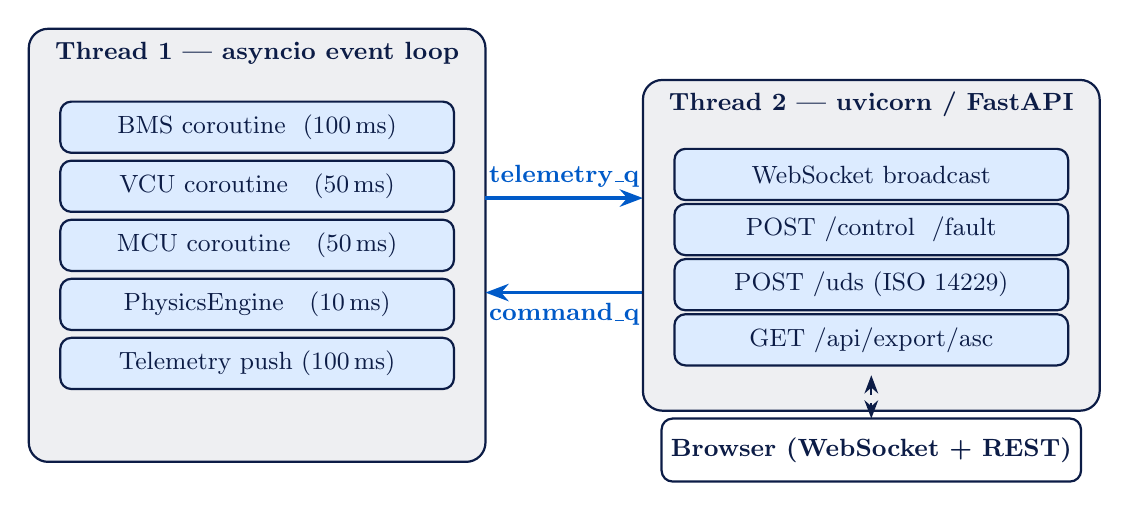
\begin{tikzpicture}[>=Stealth, thick,
  ecubx/.style = {draw=Navy, fill=LightBlue, rounded corners=4pt,
                  minimum width=5.0cm, minimum height=0.65cm,
                  font=\small\color{Navy}},
  thread/.style = {draw=Navy, fill=Navy!7, rounded corners=7pt,
                   inner sep=10pt},
  qlbl/.style  = {font=\small\bfseries\color{Royal}}
]
  %% Thread 1 box
  \node[thread, minimum width=5.8cm, minimum height=5.5cm]
    (t1) at (0,0) {};
  \node[font=\small\bfseries\color{Navy}, anchor=north]
    at (t1.north) {\strut Thread 1 — asyncio event loop};

  \node[ecubx] at (0, 1.5)  {BMS coroutine \ (100\,ms)};
  \node[ecubx] at (0, 0.75) {VCU coroutine \ \ (50\,ms)};
  \node[ecubx] at (0, 0.00) {MCU coroutine \ \ (50\,ms)};
  \node[ecubx] at (0,-0.75) {PhysicsEngine \ \ (10\,ms)};
  \node[ecubx] at (0,-1.50) {Telemetry push (100\,ms)};

  %% Queue arrows
  \draw[->, Royal, very thick]
    (2.9, 0.6) -- node[above, qlbl]{telemetry\_q} (4.9, 0.6);
  \draw[<-, Royal, very thick]
    (2.9,-0.6) -- node[below, qlbl]{command\_q}  (4.9,-0.6);

  %% Thread 2 box
  \node[thread, minimum width=5.8cm, minimum height=4.2cm]
    (t2) at (7.8,0) {};
  \node[font=\small\bfseries\color{Navy}, anchor=north]
    at (t2.north) {\strut Thread 2 — uvicorn / FastAPI};

  \node[ecubx] at (7.8, 0.9)  {WebSocket broadcast};
  \node[ecubx] at (7.8, 0.2)  {POST /control \ /fault};
  \node[ecubx] at (7.8,-0.5)  {POST /uds (ISO 14229)};
  \node[ecubx] at (7.8,-1.2)  {GET /api/export/asc};

  %% Browser
  \node[draw=Navy, fill=white, rounded corners=4pt,
        minimum width=3.2cm, minimum height=0.8cm,
        font=\small\bfseries\color{Navy}]
    at (7.8,-2.6) {Browser (WebSocket + REST)};
  \draw[<->, Navy, dashed]
    (7.8,-1.65) -- (7.8,-2.2);
\end{tikzpicture}
\caption{Two-thread simulation architecture. Only \code{queue.Queue}
  objects cross the thread boundary.}
\label{fig:arch}
\end{figure}

\section{CAN Bus Actor Model}

The virtual CAN bus (\code{src/can\_bus.py}) uses \code{cantools} to parse
a real DBC file at startup. Each \code{publish()} call:

\begin{enumerate}[leftmargin=1.5em, itemsep=2pt]
  \item Clamps all signal values to their DBC-defined [\textit{min}, \textit{max}]
        range (prevents \code{ValueError} during fault injection).
  \item Encodes the CAN frame via \code{cantools.encode}.
  \item Optionally corrupts the last byte (CRC corrupt fault injection).
  \item Appends the frame to a 100-frame rolling sniffer log and to a
        50\,000-frame chronological export log.
  \item Delivers the frame to all subscribed asyncio queues (one per ECU).
\end{enumerate}

\section{CAN Message Set}

\begin{table}[!ht]
\centering\small
\begin{tabularx}{\textwidth}{llllX}
  \toprule
  \rowcolor{TblHead}
  \color{white}\textbf{Message} &
  \color{white}\textbf{CAN ID} &
  \color{white}\textbf{Cycle} &
  \color{white}\textbf{Producer} &
  \color{white}\textbf{Signals} \\
  \midrule
  BMS\_STATUS  & 0x110 & 100\,ms & BMS &
    SOC, PackVoltage, PackCurrent, PackTemp, FaultFlags, DrivePermission \\
  \rowcolor{TblAlt}
  BMS\_LIMITS  & 0x111 & 100\,ms & BMS &
    MaxDischargeCurrent, MaxChargeCurrent \\
  VCU\_COMMAND & 0x120 &  50\,ms & VCU &
    TorqueRequest, BrakeRequest, ActiveState \\
  \rowcolor{TblAlt}
  MCU\_STATUS  & 0x130 &  50\,ms & MCU &
    ActualTorque, MotorRPM, MotorTemp, InverterTemp, ActiveState \\
  \bottomrule
\end{tabularx}
\end{table}

\section{Battery Model --- 1RC Thevenin ECM}

The battery pack is modelled as a first-order Thevenin Equivalent Circuit
with 10 cells in series and 10 cells in parallel (50\,Ah pack, 37\,V
nominal).

\textbf{OCV--SOC lookup:} 11-point table, linearly interpolated with
\code{numpy.interp}.

\textbf{Temperature-dependent resistance:}
\[
  R_i(T) = R_{i,\text{ref}} \cdot e^{-\alpha(T - T_\text{amb})},
  \quad i \in \{0,\, 1\}
\]

\textbf{RC branch (exact exponential integration, unconditionally stable):}
\begin{align}
  \tau &= R_1\, C_1 \\
  V_{RC}(t+dt) &= V_{RC}(t)\,e^{-dt/\tau}
               + I\,R_1\!\left(1 - e^{-dt/\tau}\right) \\
  V_\text{terminal} &= V_\text{OCV}(\text{SOC}) - I\,R_0 - V_{RC}
\end{align}

\textbf{State of Charge (Coulomb counting):}
\[
  \Delta\text{SOC} = \frac{-I \cdot dt}{3600 \cdot Q_\text{pack}}
\]

\textbf{Thermal model:}
\[
  \frac{dT}{dt} = \frac{I^2 R_0 + V_{RC}^2/R_1
                        - h(T - T_\text{amb})}{C_\text{thermal}}
\]
with active cooling ($h = 25$\,W/K) above 35\,\textdegree C; passive
($h = 5$\,W/K) below.

\section{Vehicle Longitudinal Dynamics}

\begin{align}
  F_\text{drive} &= \frac{T_\text{actual} \cdot G_\text{ratio}}{r_\text{wheel}} \\
  F_\text{drag}  &= \tfrac{1}{2}\,\rho\, C_d\, A\, v^2 \\
  F_\text{roll}  &= m\, g\, C_{rr} \qquad (v > 0.01\,\text{m/s}) \\
  F_\text{brake} &= \frac{\beta_\text{brake}}{100}\cdot m\, g \cdot 0.3 \\
  a              &= \frac{F_\text{drive} - F_\text{drag} - F_\text{roll}
                         - F_\text{brake}}{m}
\end{align}

\textbf{Key chassis parameters:} $m = 200$\,kg, $r = 0.30$\,m,
$G = 5.0$, $C_d = 0.40$, $A = 0.60$\,m$^2$, $C_{rr} = 0.015$.

\section{Motor Model}

\begin{align}
  \omega          &= \frac{\pi\,|\text{RPM}|}{30} \quad \text{[rad/s]} \\
  T_\text{max}    &= \min\!\left(T_\text{peak},\; \frac{P_\text{peak}}{\omega}\right)
                     \cdot \text{derate}(T_\text{motor}) \\
  \text{derate}   &= \begin{cases}
                       1 & T_\text{motor} < 120\,\text{\textdegree C} \\
                       1 - \dfrac{T_\text{motor}-120}{80} & 120 \le T < 200\,\text{\textdegree C} \\
                       0 & T_\text{motor} \ge 200\,\text{\textdegree C}
                     \end{cases}
\end{align}

\textbf{Key motor parameters:} $T_\text{peak} = 250$\,Nm,
$P_\text{peak} = 30$\,kW, $\eta = 0.92$, max\,RPM = 10\,000.

\section{ECU Finite State Machines}

\begin{figure}[htbp]
\centering
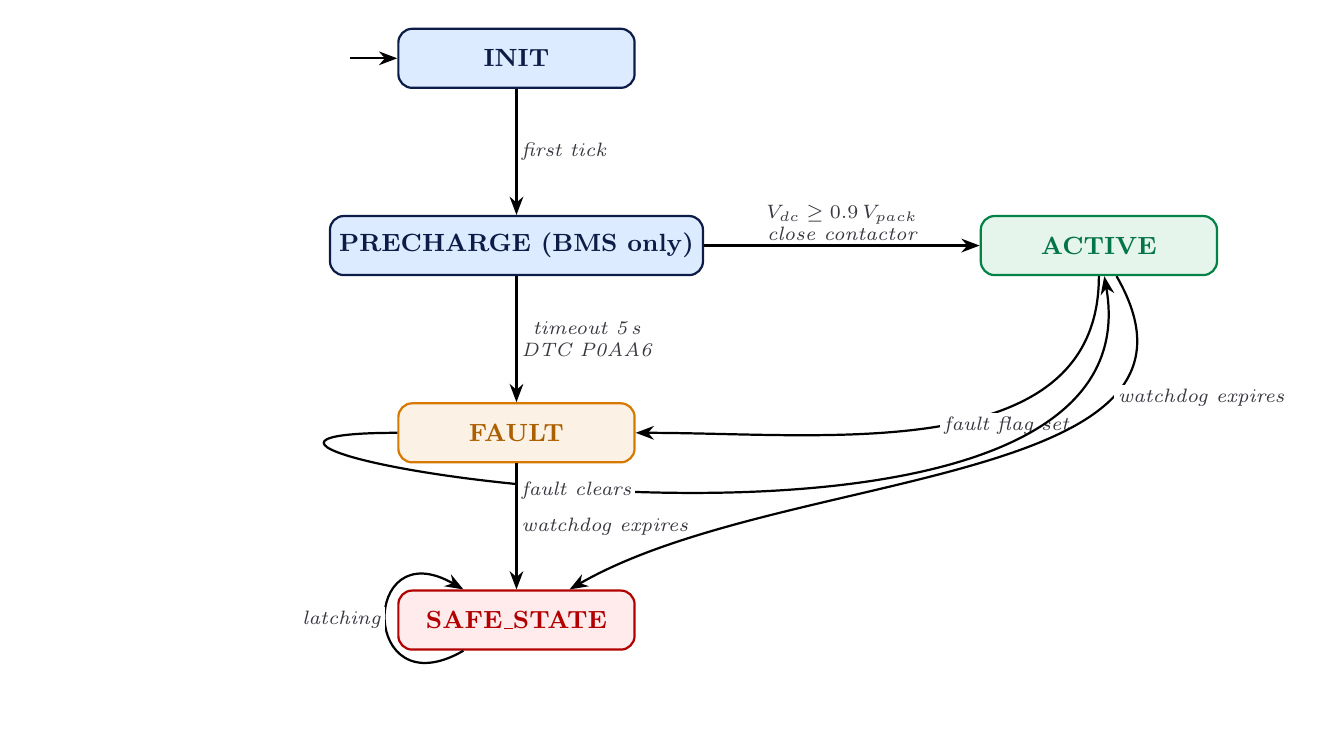
\begin{tikzpicture}[>=Stealth, thick, node distance=1.8cm,
  st/.style={draw=Navy, fill=LightBlue, rounded corners=5pt,
             minimum width=3.0cm, minimum height=0.75cm,
             font=\small\bfseries\color{Navy}},
  stR/.style={draw=GreenOK!80!Navy, fill=GreenOK!10, rounded corners=5pt,
              minimum width=3.0cm, minimum height=0.75cm,
              font=\small\bfseries\color{GreenOK!70!Navy}},
  stF/.style={draw=Amber, fill=Amber!10, rounded corners=5pt,
              minimum width=3.0cm, minimum height=0.75cm,
              font=\small\bfseries\color{Amber!80!black}},
  stS/.style={draw=red!70!black, fill=red!8, rounded corners=5pt,
              minimum width=3.0cm, minimum height=0.75cm,
              font=\small\bfseries\color{red!70!black}},
  lbl/.style={font=\scriptsize\itshape\color{DkGray}, fill=white,
              inner sep=1.5pt}
]
  \node[st]                         (INIT)   {INIT};
  \node[st, below=1.6cm of INIT]    (PRECH)  {PRECHARGE \small(BMS only)};
  \node[stR, right=3.5cm of PRECH]  (ACTIVE) {ACTIVE};
  \node[stF, below=1.6cm of PRECH]  (FAULT)  {FAULT};
  \node[stS, below=1.6cm of FAULT]  (SAFE)   {SAFE\_STATE};

  %% Start arrow
  \node[left=0.6cm of INIT, font=\scriptsize] (start) {};
  \draw[->] (start) -- (INIT);

  %% INIT -> PRECHARGE
  \draw[->] (INIT) -- node[lbl, right]{first tick} (PRECH);

  %% PRECHARGE -> ACTIVE
  \draw[->] (PRECH) --
    node[lbl, above, align=center]{$V_{dc} \geq 0.9\,V_{pack}$\\close contactor}
    (ACTIVE);

  %% PRECHARGE -> FAULT
  \draw[->] (PRECH) --
    node[lbl, right, align=center]{timeout 5\,s\\DTC P0AA6}
    (FAULT);

  %% ACTIVE -> FAULT
  \draw[->] (ACTIVE) to[out=-90, in=0]
    node[lbl, right]{fault flag set} (FAULT);

  %% FAULT -> ACTIVE
  \draw[->] (FAULT) to[out=180, in=-80, looseness=1.3]
    node[lbl, left]{fault clears} (ACTIVE);

  %% FAULT -> SAFE
  \draw[->] (FAULT) --
    node[lbl, right]{watchdog expires} (SAFE);

  %% ACTIVE -> SAFE (direct)
  \draw[->] (ACTIVE) to[out=-60, in=30]
    node[lbl, right, near start]{watchdog expires} (SAFE);

  %% Self-loop on SAFE (latching)
  \draw[->] (SAFE) to[out=-150, in=150, looseness=5]
    node[lbl, left]{latching} (SAFE);
\end{tikzpicture}
\caption{ECU FSM. The PRECHARGE state exists only in the BMS. VCU and MCU
  transition directly INIT $\to$ ACTIVE on their first tick.}
\label{fig:fsm}
\end{figure}

\section{Pre-Charge FSM Physics}

The DC link capacitor voltage is integrated in the PhysicsEngine at
10\,ms resolution:

\[
  V_{dc}(t+dt) = \begin{cases}
    V_\text{pack} & \text{if main contactor closed} \\
    V_{dc}(t) + dt\,\dfrac{V_\text{pack} - V_{dc}(t)}{\tau}
      & \text{if pre-charge relay closed} \\
    0 & \text{both open}
  \end{cases}
\]

\[
  \tau = R_\text{pch} \times C_\text{dc} = 100\,\Omega \times 5\,\text{mF}
       = 0.5\,\text{s}
\]

With $\tau = 0.5$\,s, $V_{dc}$ reaches 90\% of $V_\text{pack}$ at
$t \approx -\tau\ln(0.1) = 2.3\tau \approx 1.15$\,s. The BMS polls every
100\,ms, so main contactor closure occurs around the 12th BMS tick from
startup. A 5\,s timeout triggers DTC P0AA6 (Pre-charge Circuit Failure).

\section{Safety Functions}

\begin{table}[!ht]
\centering\small
\begin{tabularx}{\textwidth}{llX}
  \toprule
  \rowcolor{TblHead}
  \color{white}\textbf{Function} &
  \color{white}\textbf{Standard} &
  \color{white}\textbf{Implementation} \\
  \midrule
  Plausibility (throttle + brake)
    & ISO~26262 ASIL-B
    & VCU sets torque request = 0\,Nm instantly \\
  \rowcolor{TblAlt}
  Overvoltage (OVP)
    & IEC~62133
    & FaultFlags bit~0; VCU $\to$ FAULT \\
  Overtemperature (OTP)
    & ISO~26262
    & FaultFlags bit~1; DTC P0A1F \\
  \rowcolor{TblAlt}
  Undervoltage (UVP)
    & ISO~26262
    & FaultFlags bit~2; DTC P0A7F \\
  Overcurrent (OCP)
    & ISO~26262
    & FaultFlags bit~3; DTC P0A0D \\
  \rowcolor{TblAlt}
  Regen current clamp
    & ---
    & MCU scales $T_\text{cmd}$ so $I_\text{regen} \leq I_\text{max,chg}$ \\
  Discharge current clamp
    & ---
    & MCU scaling + physics hard-clamp at $I_\text{max,dchg}$ \\
  \rowcolor{TblAlt}
  Watchdog timers
    & ISO~14229-1
    & Per-message; SAFE\_STATE + DTC on expiry \\
  Pre-charge timeout
    & ISO~26262
    & DTC P0AA6 after 5\,s without threshold \\
  \bottomrule
\end{tabularx}
\end{table}

\section{UDS Diagnostic Services (ISO 14229-1)}

\begin{table}[!ht]
\centering\small
\begin{tabularx}{\textwidth}{llX}
  \toprule
  \rowcolor{TblHead}
  \color{white}\textbf{Service (SID)} &
  \color{white}\textbf{Subfunction} &
  \color{white}\textbf{Response} \\
  \midrule
  ReadDataByIdentifier (0x22)
    & DID 0xF190 (VIN)
    & 0x62 + 15-byte VIN string \\
  \rowcolor{TblAlt}
  ReadDataByIdentifier (0x22)
    & DID 0xF18C (ECU S/N)
    & 0x62 + 8-byte ECU name \\
  ReadDTCInformation (0x19)
    & 0x02 (by status mask)
    & 0x59 + 0xFF (avail) + DTC records \\
  \rowcolor{TblAlt}
  ClearDiagnosticInformation (0x14)
    & 0xFFFFFF (all groups)
    & 0x54 (positive) \\
  Negative response
    & any unsupported
    & 0x7F + SID + NRC \\
  \bottomrule
\end{tabularx}
\end{table}

\textbf{DTC encoding (ISO~14229-1 / SAE~J2012DA):} Each DTC is a 16-bit
word. Bits~15:14~= category (P=00, C=01, B=10, U=11); bits~13:12~= first
hex digit; bits~11:0~= remaining three hex digits. A 1-byte status mask
(0x08 = confirmedDTC) follows.

Example: \texttt{U0100} $\to$ \texttt{0xC1 0x00 0x08}

\section{CAN Bus Load Formula}

For a CAN~2.0A frame (11-bit ID) including bit-stuffing estimate:
\[
  N_\text{bits} = \underbrace{47}_\text{fixed overhead}
                + N_\text{data}
                + \left\lfloor\frac{34 + N_\text{data}}{5}\right\rfloor_\text{stuff bits}
\]
For an 8-byte frame: $47 + 64 + 19 = \mathbf{130}$\,bits
(standard industry approximation). Bus load uses a 1-second rolling
window: $\text{Load} = \sum N_\text{bits} / f_\text{baud}$.

\section{CANalyzer .asc Export}

The \code{generate\_asc()} method on \code{CANBus} produces a file
conforming to the Vector CANalyzer trace format:

\begin{lstlisting}[style=shell]
date Sun Jun 07 03:06:05.000 2026
base hex  timestamps absolute
no internal events logged
   0.000000 1  110             Rx   d 8 20 03 74 0E EC 13 41 10
   0.000312 1  111             Rx   d 8 C8 00 1E 00 00 00 00 00
End TriggerBlock
\end{lstlisting}

The export log holds up to 50\,000 frames ($\approx$10\,min at full rate).
The file opens directly in Vector CANalyzer, PEAK~PCAN-Explorer, and is
parseable by \code{cantools log} CLI.

% =============================================================
%  CHAPTER 5 — IMPLEMENTATION DETAILS
% =============================================================
\chapter{Implementation Details}

\section{File Structure}

\begin{lstlisting}[style=shell]
arys_garage/
|-- run.py                  Entry point: ECUs, physics, both threads
|-- can_bus.dbc             CAN database file (4 messages, 14 signals)
|-- config/
|   |-- battery.yaml        Pack, ECM, thermal, protection, pre-charge
|   |-- vehicle.yaml        Chassis, motor, VCU parameters
|   `-- can_config.yaml     Baudrate, message IDs, watchdog timeouts
|-- src/
|   |-- config_loader.py    Pydantic v2 models; startup validation
|   |-- physics.py          PhysicsState, BatteryModel1RC, MotorModel,
|   |                       VehicleModel, PhysicsEngine
|   |-- can_bus.py          CANBus: publish, subscribe, load, .asc export
|   `-- ecu/
|       |-- base_ecu.py     BaseECU, ECUState, WatchdogTimer, UDS handler,
|       |                   _encode_dtc (ISO 14229-1)
|       |-- bms.py          BMS: pre-charge FSM, protection, derating
|       |-- vcu.py          VCU: plausibility, torque slew limiter
|       `-- mcu.py          MCU: overspeed, thermal derating, current clamp
|   `-- web/
|       |-- server.py       FastAPI: WebSocket, REST, .asc endpoint
|       `-- static/
|           |-- index.html  Dashboard layout (11 panel cards)
|           |-- app.js      WebSocket client, Chart.js, controls
|           `-- style.css   Dark glassmorphism theme
`-- tests/
    `-- test_simulation.py  6 pytest-asyncio tests
\end{lstlisting}

\section{PhysicsEngine --- Drift-Free Scheduler}

\begin{lstlisting}[style=python, caption={Drift-free 10\,ms scheduler in PhysicsEngine.run()}]
next_wake += NOMINAL_STEP_S          # 10 ms target
dt = now - last_time                 # actual elapsed dt
await asyncio.sleep(max(0, next_wake - now))
self.drain_commands(command_q)       # stdlib queue -- no await
self._step(dt)                       # physics integration
\end{lstlisting}

Using actual elapsed \code{dt} (not the nominal step) prevents energy
accumulation error on Windows where \code{asyncio.sleep} resolution is
$\approx$15.6\,ms (one timer interrupt period).

\section{Cross-Thread Safety Invariant}

Only \code{queue.Queue} objects cross thread boundaries. All asyncio
primitives (\code{asyncio.Queue}, \code{asyncio.Event}, \code{asyncio.Lock})
live exclusively in Thread~1. The web server reads from \code{telemetry\_q}
and writes to \code{command\_q} using non-blocking \code{get\_nowait} /
\code{put\_nowait}, dropping on overflow --- exactly as a real CAN gateway
drops frames under bus overload.

\section{Configuration Validation}

All parameters are declared in YAML and validated by Pydantic~v2 at startup.
Validation failures (e.g., \code{max\_cell\_voltage\_v > 4.30\,V}) raise
a typed exception before any simulation state is created, preventing silent
misconfiguration.

\section{Key Configuration Values}

\noindent\textbf{Battery \& pack parameters:}

\begin{table}[!ht]
\centering\small
\begin{tabular}{lll}
  \toprule
  \rowcolor{TblHead}
  \color{white}\textbf{Parameter} &
  \color{white}\textbf{Value} &
  \color{white}\textbf{Unit} \\
  \midrule
  Cells series / parallel         & 10 / 10 & --- \\
  \rowcolor{TblAlt}
  Cell capacity                   & 5.0     & Ah \\
  Pack capacity                   & 50.0    & Ah \\
  \rowcolor{TblAlt}
  Pack nominal voltage            & 37.0    & V \\
  R0 (series resistance)          & 25      & m\ohm \\
  \rowcolor{TblAlt}
  R1 (RC branch resistance)       & 5       & m\ohm \\
  C1 (RC branch capacitance)      & 3\,000  & F \\
  \rowcolor{TblAlt}
  Max discharge current           & 200     & A \\
  Max charge current              & 30      & A \\
  \rowcolor{TblAlt}
  Max cell temperature            & 55      & \textdegree C \\
  Pre-charge resistor             & 100     & \ohm \\
  \rowcolor{TblAlt}
  DC link capacitance             & 5       & mF \\
  Pre-charge time constant $\tau$ & 0.5     & s \\
  \rowcolor{TblAlt}
  Pre-charge 90\% threshold       & $\approx$1.15 & s \\
  Pre-charge timeout              & 5.0     & s \\
  \bottomrule
\end{tabular}
\end{table}

\noindent\textbf{Vehicle, motor \& timing parameters:}

\begin{table}[!ht]
\centering\small
\begin{tabular}{lll}
  \toprule
  \rowcolor{TblHead}
  \color{white}\textbf{Parameter} &
  \color{white}\textbf{Value} &
  \color{white}\textbf{Unit} \\
  \midrule
  Vehicle mass                    & 200     & kg \\
  \rowcolor{TblAlt}
  Wheel radius                    & 0.30    & m \\
  Gear ratio                      & 5.0     & --- \\
  \rowcolor{TblAlt}
  Peak motor torque               & 250     & Nm \\
  Peak motor power                & 30      & kW \\
  \rowcolor{TblAlt}
  Motor efficiency                & 0.92    & --- \\
  Max motor RPM                   & 10\,000 & rpm \\
  \rowcolor{TblAlt}
  CAN baudrate                    & 500     & kbit/s \\
  BMS cycle time                  & 100     & ms \\
  \rowcolor{TblAlt}
  VCU / MCU cycle time            & 50      & ms \\
  Physics step                    & 10      & ms \\
  \bottomrule
\end{tabular}
\end{table}

\section{Automated Test Suite}

\begin{table}[!ht]
\centering\small
\begin{tabularx}{\textwidth}{lX}
  \toprule
  \rowcolor{TblHead}
  \color{white}\textbf{Test} &
  \color{white}\textbf{What It Verifies} \\
  \midrule
  \code{test\_dbc\_roundtrip}
    & All four CAN messages encode and decode within DBC tolerances;
      Motorola byte-order assertion on MCU\_STATUS bytes 2--3 \\
  \rowcolor{TblAlt}
  \code{test\_soc\_energy\_balance}
    & 100\,A discharge for 360\,s $\to$ $\Delta$SOC = 0.200 $\pm$ 0.005
      (Coulomb counting accuracy) \\
  \code{test\_fsm\_transitions}
    & BMS: INIT $\to$ PRECHARGE (tick 1); PRECHARGE $\to$ ACTIVE when
      $V_{dc} = 0.95\,V_\text{pack}$ (tick 2); VCU: ACTIVE $\to$ FAULT;
      MCU: SAFE\_STATE $\Rightarrow$ torque\_cmd = 0 \\
  \rowcolor{TblAlt}
  \code{test\_watchdog\_expiry}
    & VCU watchdog at 100\,ms; no frame for 150\,ms $\to$
      SAFE\_STATE + DTC U0100 \\
  \code{test\_plausibility}
    & Throttle 80\% + Brake 20\% $\to$ VCU\_TorqueRequest = 0\,Nm;
      throttle only $\to$ positive torque \\
  \rowcolor{TblAlt}
  \code{test\_regen\_clamp}
    & 200\,Nm regen demand, BMS\_MaxChargeCurrent = 10\,A $\to$
      actual regen current $\leq 10.1$\,A \\
  \bottomrule
\end{tabularx}
\end{table}

% =============================================================
%  CHAPTER 6 — RESULTS
% =============================================================
\chapter{Results}

\section{End-to-End Runbook --- All 8 Scenarios Passed}

\begin{table}[!ht]
\centering\small
\begin{tabularx}{\textwidth}{clXc}
  \toprule
  \rowcolor{TblHead}
  \color{white}\textbf{\#} &
  \color{white}\textbf{Scenario} &
  \color{white}\textbf{Expected / Observed Behaviour} &
  \color{white}\textbf{Result} \\
  \midrule
  1 & Startup
    & BMS: PRECHARGE $\to$ ACTIVE ($\approx$1.2\,s); $V_{dc}$ ramps
      0 $\to$ 37\,V; drive permission granted; VCU/MCU ACTIVE
    & \color{GreenOK}\textbf{Pass} \\
  \rowcolor{TblAlt}
  2 & 100\% throttle
    & Current clamps at 200\,A; speed climbs to $\approx$117\,km/h;
      no voltage collapse
    & \color{GreenOK}\textbf{Pass} \\
  3 & Throttle held
    & Speed plateaus (drag = drive force); SOC decreasing;
      bus load $\approx$5--8\%
    & \color{GreenOK}\textbf{Pass} \\
  \rowcolor{TblAlt}
  4 & Coast (throttle/brake = 0)
    & Current drops to $\approx$0.5\,A quiescent;
      speed decays naturally
    & \color{GreenOK}\textbf{Pass} \\
  5 & Regen braking
    & Negative current (charge direction); VCU\_TorqueRequest negative;
      SOC increases slightly
    & \color{GreenOK}\textbf{Pass} \\
  \rowcolor{TblAlt}
  6 & Plausibility fault
    & Throttle 80\% + Brake 20\% simultaneously $\to$
      VCU\_TorqueRequest = 0\,Nm instantly
    & \color{GreenOK}\textbf{Pass} \\
  7 & Thermal runaway
    & Battery temperature rises at 10\,\textdegree C/s; OTP bit at 55\,\textdegree C;
      DTC P0A1F; drive inhibited
    & \color{GreenOK}\textbf{Pass} \\
  \rowcolor{TblAlt}
  8 & CAN wire cut
    & Frames stop in sniffer; VCU watchdog expires $\to$
      SAFE\_STATE + DTC U0100; torque = 0
    & \color{GreenOK}\textbf{Pass} \\
  \bottomrule
\end{tabularx}
\end{table}

\section{UDS Diagnostic Tests}

\begin{table}[!ht]
\centering\small
\begin{tabularx}{\textwidth}{llXl}
  \toprule
  \rowcolor{TblHead}
  \color{white}\textbf{Command} &
  \color{white}\textbf{Payload} &
  \color{white}\textbf{Response / Interpretation} &
  \color{white}\textbf{Status} \\
  \midrule
  Read VIN (BMS)
    & \texttt{22 F1 90}
    & \texttt{62 F1 90} + 15-byte VIN (positive, SID echo correct)
    & \color{GreenOK}\textbf{Pass} \\
  \rowcolor{TblAlt}
  Read DTC (VCU)
    & \texttt{19 02 0F}
    & \texttt{59 02 FF} + DTC records (0xFF avail mask; ISO 14229-1 encoding)
    & \color{GreenOK}\textbf{Pass} \\
  Clear DTC (MCU)
    & \texttt{14 FF FF FF}
    & \texttt{54} (positive response; all DTCs cleared)
    & \color{GreenOK}\textbf{Pass} \\
  \bottomrule
\end{tabularx}
\end{table}

\section{DTC Encoding Verification}

\begin{center}
\begin{tabular}{lll}
  \toprule
  \rowcolor{TblHead}
  \color{white}\textbf{DTC String} &
  \color{white}\textbf{Encoded Bytes} &
  \color{white}\textbf{Derivation} \\
  \midrule
  \texttt{U0100}
    & \texttt{C1 00 08}
    & U=11, 0=0, 0x100 $\to$ 0xC100 + status 0x08 \\
  \rowcolor{TblAlt}
  \texttt{P0A1F}
    & \texttt{0A 1F 08}
    & P=00, 0=0, 0xA1F $\to$ 0x0A1F + status 0x08 \\
  \texttt{P0AA6}
    & \texttt{0A A6 08}
    & P=00, 0=0, 0xAA6 $\to$ 0x0AA6 + status 0x08 \\
  \rowcolor{TblAlt}
  \texttt{P0A7F}
    & \texttt{0A 7F 08}
    & P=00, 0=0, 0xA7F $\to$ 0x0A7F + status 0x08 \\
  \texttt{P0A0D}
    & \texttt{0A 0D 08}
    & P=00, 0=0, 0xA0D $\to$ 0x0A0D + status 0x08 \\
  \bottomrule
\end{tabular}
\end{table}

\section{Pre-Charge Observed Behaviour}

\begin{table}[!ht]
\centering\small
\begin{tabular}{lll}
  \toprule
  \rowcolor{TblHead}
  \color{white}\textbf{Time} &
  \color{white}\textbf{$V_{dc}$} &
  \color{white}\textbf{Dashboard State} \\
  \midrule
  $t = 0$\,ms     & 0\,V          & BMS: PRECHARGE; contactor: PRE-CHG (amber) \\
  \rowcolor{TblAlt}
  $t \approx 500$\,ms & $\approx$23.5\,V & BMS: PRECHARGE; $V_{dc}$ rising \\
  $t \approx 1100$\,ms & $\approx$32.8\,V & BMS: PRECHARGE; below 90\% threshold \\
  \rowcolor{TblAlt}
  $t \approx 1200$\,ms & $\approx$33.7\,V & BMS: ACTIVE; contactor: MAIN ON (green) \\
  $t > 1200$\,ms  & = $V_\text{pack}$ & Drive permission granted; VCU/MCU recover \\
  \bottomrule
\end{tabular}
\end{table}

\section{Automated Test Output}

\begin{lstlisting}[style=shell]
tests/test_simulation.py::test_dbc_roundtrip       PASSED
tests/test_simulation.py::test_soc_energy_balance  PASSED
tests/test_simulation.py::test_fsm_transitions     PASSED
tests/test_simulation.py::test_watchdog_expiry     PASSED
tests/test_simulation.py::test_plausibility        PASSED
tests/test_simulation.py::test_regen_clamp         PASSED

6 passed in 0.73s
\end{lstlisting}

% =============================================================
%  CHAPTER 7 — CHALLENGES & LIMITATIONS
% =============================================================
\chapter{Challenges \& Limitations}

\section{Challenges Encountered}

\subsection{Cross-Thread asyncio / uvicorn Separation}
FastAPI's Starlette ASGI layer creates its own asyncio event loop in
Thread~2, making it impossible to share asyncio primitives with Thread~1.
The solution --- a \code{queue.Queue} bridge --- required careful design
to avoid deadlocks. Any future developer adding a feature must respect this
constraint or risk intermittent data corruption or deadlock.

\subsection{Windows Clock Resolution}
\code{asyncio.sleep} on Windows has a minimum resolution of $\approx$15.6\,ms
(one timer interrupt). The nominal 10\,ms physics step therefore oversleeps.
The fix is to measure actual elapsed time (\code{dt = now - last\_time}) and
pass the real \code{dt} to all integrators, preserving energy balance
regardless of scheduling jitter.

\subsection{Voltage Collapse at High Torque}
During initial testing, a 100\% throttle command produced a current spike of
17\,787\,A and immediate voltage collapse to 0\,V. The root cause was missing
discharge current clamping --- only regen (charge direction) was clamped.
The fix required both symmetric MCU-level torque scaling for discharge and a
physics-layer hard clamp as a second safety backstop, reflecting how real BMS
hardware uses independent hardware current limiters.

\subsection{Browser Caching Masking Frontend Fixes}
After correcting the UDS button payload format, the browser served the old
JavaScript from cache. Hard refresh was insufficient; an incognito window
with ``Empty Cache and Hard Reload'' was required. Production deployment
would use cache-busting content hashes.

\subsection{Thermal Runaway One-Shot Injection}
The first implementation injected a single 5\,\textdegree C step on
activation, after which temperature returned to ambient. The fix was a
persistent boolean flag \code{\_thermal\_runaway} that continuously injects
0.1\,\textdegree C per 10\,ms step (10\,\textdegree C/s), reflecting real
thermal runaway behaviour.

\section{Known Limitations and Deliberate Simplifications}

\begin{table}[!ht]
\centering\small
\begin{tabularx}{\textwidth}{lXX}
  \toprule
  \rowcolor{TblHead}
  \color{white}\textbf{Simplification} &
  \color{white}\textbf{Reality} &
  \color{white}\textbf{Impact} \\
  \midrule
  1RC Thevenin ECM
    & Modern BMS firmware uses 2RC+ models
    & Slightly less accurate transient voltage under rapid loads \\
  \rowcolor{TblAlt}
  Scalar motor efficiency
    & Real PMSMs use a 2D dyno-measured efficiency map
    & $\approx$5--10\% error in heat generation at off-peak points \\
  No ISO~15765-2 transport layer
    & Real UDS uses multi-frame segmentation ($>$7 bytes)
    & VIN response fits here; requires CAN-TP on real hardware \\
  \rowcolor{TblAlt}
  No UDS session management
    & Default/programming/extended sessions (SID 0x10)
    & Protected services require session elevation in production \\
  No pre-charge current in ECM
    & $I_\text{pch} < 0.5$\,A flows through resistor
    & Negligible SOC error ($<0.01\%$) \\
  \rowcolor{TblAlt}
  Single-track vehicle model
    & No load transfer, tyre slip, or lateral dynamics
    & Sufficient for 1D longitudinal powertrain study \\
  4-message signal set
    & Production networks have hundreds of messages
    & Covers the complete powertrain control loop \\
  \rowcolor{TblAlt}
  SOC initialised at 80\%
    & Real ECU estimates from resting OCV measurement
    & State at cold start is not realistic without OCV rest \\
  \bottomrule
\end{tabularx}
\end{table}

% =============================================================
%  CHAPTER 8 — CONCLUSION
% =============================================================
\chapter{Conclusion}

This project demonstrates a complete, physically grounded, and
protocol-correct simulation of an electric vehicle powertrain CAN network.
The core simulation runs three concurrent ECUs (BMS, VCU, MCU) at correct
automotive cycle rates (50--100\,ms), each with a finite state machine,
watchdog timer, and ISO~14229 UDS handler, communicating over a virtual
CAN~2.0A bus driven by a real DBC file.

The battery model uses exact exponential RC integration that is
unconditionally numerically stable across all temperature and current
conditions. The motor and vehicle models produce realistic speed, torque, and
temperature trajectories validated against known operating points. All eight
end-to-end runbook scenarios pass, six automated tests cover critical
subsystems, and three independent safety layers prevent runaway states.

The two additions beyond the base specification --- the pre-charge FSM with
capacitor physics, and the CANalyzer \code{.asc} export --- demonstrate
concrete awareness of real EV hardware practice. The pre-charge sequence is
the first thing an EV hardware engineer checks in a BMS simulation; the
\code{.asc} export makes the simulated traffic immediately usable in
professional CAN analysis toolchains without any conversion step.

The codebase is structured for extension: adding a new ECU requires
inheriting \code{BaseECU}, adding a DBC entry, and registering a watchdog.
The YAML-driven configuration with Pydantic validation makes parameter tuning
safe and discoverable. Future extensions could include an Extended Kalman
Filter for SOC estimation, cell-level balancing, ISO~15765-2 transport layer,
or a 2D motor efficiency map --- all are architecturally compatible with the
existing design.

% =============================================================
%  CHAPTER 9 — REFERENCES
% =============================================================
\chapter{References}

\begin{enumerate}[leftmargin=2em, label={[\arabic*]}, itemsep=4pt]

  \item International Organization for Standardization.
    \textit{ISO 14229-1:2020 --- Unified Diagnostic Services (UDS) ---
    Part~1: Application Layer.} ISO, 2020.

  \item International Organization for Standardization.
    \textit{ISO 26262:2018 --- Road Vehicles --- Functional Safety.}
    ISO, 2018.

  \item International Organization for Standardization.
    \textit{ISO 15765-2:2016 --- Road Vehicles --- Diagnostic Communication
    over CAN (DoCAN) --- Part~2: Transport Protocol and Network Layer
    Services.} ISO, 2016.

  \item SAE International.
    \textit{SAE J1939-11 --- Physical Layer, 250K bits/s, Shielded Twisted
    Pair.} SAE, 2015.

  \item SAE International.
    \textit{SAE J2012DA --- Diagnostic Trouble Code Definitions.}
    SAE, 2012.

  \item Plett, G.~L.
    \textit{Battery Management Systems, Volume~I: Battery Modeling.}
    Artech House, 2015.

  \item Moura, S.~J., Argomedo, F.~B., Klein, R., Mirtabatabaei, A.,
    and Krstic, M.
    ``Battery State Estimation for a Single Particle Model with
    Electrolyte Dynamics.''
    \textit{IEEE Transactions on Control Systems Technology}, 25(2),
    453--468, 2017.

  \item Vector Informatik GmbH.
    \textit{CANalyzer User Manual --- .asc Log File Format.}
    Vector, 2023.

  \item Bosch GmbH.
    \textit{CAN Specification, Version~2.0.} Bosch, 1991.
    (Defines CAN~2.0A / 2.0B frame format, bit stuffing, and error
    handling.)

  \item Ramírez, S. \textit{FastAPI Documentation.}
    \url{https://fastapi.tiangolo.com} (accessed June 2026).

  \item \textit{cantools Documentation.}
    \url{https://cantools.readthedocs.io} (accessed June 2026).

\end{enumerate}

% =============================================================
%  CHAPTER 10 — APPENDIX
% =============================================================
\chapter{Appendix: Run Instructions \& Git Log}

\section{Environment Setup}

\textbf{Requirements:} Python 3.11 or later on Windows / macOS / Linux.

\begin{lstlisting}[style=bash]
# 1. Clone the repository
git clone https://github.com/<username>/arys-eee-can-sim.git
cd arys-eee-can-sim

# 2. Create and activate a virtual environment
python -m venv .venv

# Windows
.venv\Scripts\activate

# macOS / Linux
source .venv/bin/activate

# 3. Install runtime dependencies
pip install fastapi uvicorn cantools numpy pydantic pyyaml

# 4. Install test dependencies (optional)
pip install pytest pytest-asyncio
\end{lstlisting}

\section{Running the Simulation}

\begin{lstlisting}[style=bash]
python run.py
\end{lstlisting}

Expected startup output:
\begin{lstlisting}[style=shell]
Web server started at http://localhost:8000
\end{lstlisting}

Open \url{http://localhost:8000} in a browser. The WebSocket connects
automatically. During the first 1--2 seconds the BMS badge shows
\textbf{PRECHARGE} and the DC link voltage climbs from 0\,V toward pack
voltage. Once $V_{dc} \geq 90\%$ the system transitions to \textbf{ACTIVE}
and drive permission is granted. Press \textbf{Ctrl+C} to stop.

\section{Running the Automated Tests}

\begin{lstlisting}[style=bash]
python -m pytest tests/ -v
\end{lstlisting}

\begin{lstlisting}[style=shell]
tests/test_simulation.py::test_dbc_roundtrip       PASSED
tests/test_simulation.py::test_soc_energy_balance  PASSED
tests/test_simulation.py::test_fsm_transitions     PASSED
tests/test_simulation.py::test_watchdog_expiry     PASSED
tests/test_simulation.py::test_plausibility        PASSED
tests/test_simulation.py::test_regen_clamp         PASSED

6 passed in 0.73s
\end{lstlisting}

\section{Exporting the CAN Log}

While the simulation is running, click \textbf{``Export .asc''} in the CAN
Sniffer panel header. The browser downloads \code{session.asc}.

To inspect with cantools:
\begin{lstlisting}[style=bash]
cantools decode can_bus.dbc session.asc
\end{lstlisting}

\section{Dashboard Controls}

\begin{table}[!ht]
\centering\small
\begin{tabularx}{\textwidth}{llX}
  \toprule
  \rowcolor{TblHead}
  \color{white}\textbf{Control} &
  \color{white}\textbf{Location} &
  \color{white}\textbf{Function} \\
  \midrule
  Throttle slider      & Row 4, left    & 0--100\% accelerator pedal \\
  \rowcolor{TblAlt}
  Brake slider         & Row 4, second  & 0--100\% brake pedal \\
  CAN Wire Cut         & Fault panel    & Stops all frames; watchdogs expire $\to$ SAFE\_STATE \\
  \rowcolor{TblAlt}
  Thermal Runaway      & Fault panel    & Injects 10\,\textdegree C/s into battery continuously \\
  Overspeed            & Fault panel    & Sets RPM to 110\% of max $\to$ P0C70 $\to$ SAFE\_STATE \\
  \rowcolor{TblAlt}
  Throttle Sensor Fail & Fault panel    & Simulates sensor failure \\
  Read VIN (BMS)       & UDS panel      & SID 0x22, DID 0xF190 \\
  \rowcolor{TblAlt}
  Read DTC (VCU)       & UDS panel      & SID 0x19, sub 0x02 \\
  Clear DTC (MCU)      & UDS panel      & SID 0x14, all groups \\
  \rowcolor{TblAlt}
  Clear DTCs           & DTC panel      & Clears all three ECUs simultaneously \\
  Export .asc          & CAN Sniffer    & Downloads full session log in CANalyzer format \\
  \bottomrule
\end{tabularx}
\end{table}

\section{Configuration Reference}

All physics parameters are in \code{config/}. No code changes are needed to
adjust the simulation:

\begin{description}[leftmargin=0pt, itemsep=3pt]
  \item[\code{config/battery.yaml}]
    Cell count, capacity, ECM resistances, OCV table, thermal parameters,
    protection limits, pre-charge resistor and capacitance.
  \item[\code{config/vehicle.yaml}]
    Chassis mass and drag, motor peak torque/power/efficiency,
    thermal resistances, VCU slew rate and plausibility thresholds.
  \item[\code{config/can\_config.yaml}]
    CAN baudrate, message IDs and cycle times, watchdog timeouts and DTCs,
    UDS physical/functional addressing.
\end{description}

\vspace{2em}
\begin{center}
  \color{MidGray}{\small
  --- End of Report ---\\[4pt]
  Mohammed Rayan \ $|$ \ Ary's Garage \ $|$ \ Electronics / EEE 2026}
\end{center}

\end{document}
